\section{\personFloer{}边界算子的\termAnomaly{}}
\label{sec:anomaly-floer-boundary-operator}

本节考察单调拉格朗日子流形对子 $(L_0,L_1)$ 的\personFloer{}边界之构造。特别地，我们分析
(13.9.28) 中低虚维数——即\personMaslov{}--\personViterbo{}指标为 $0,1,2$——的\personFloer{}模空间结构。
记
\[
 \widetilde{\mathcal M}([\ell_p,w],[\ell_q,w'])
\]
为光滑\personFloer{}流线的集合，即并集
\[
 \widetilde{\mathcal M}([\ell_p,w],[\ell_q,w'])
 :=\bigcup_{w\#B\simeq w'}\widetilde{\mathcal M}(p,q;B),
\]
其中 $\widetilde{\mathcal M}(p,q;B)$ 是先前定义的连接 $p,q\in L_0\cap L_1$、满足
$[u]=B\in\pi_2(p,q)$ 的光滑\personFloer{}流线集合。

\subsection{\personFloer{} \termPreBoundaryMap{}的定义}
\label{subsec:floer-pre-boundary-definition}

先注意，若\termMonotonicityConstant{}为正，且 $\beta$ 容许一个非常值伪全纯圆盘，则
$\mu(\beta)>0$。从如下引理开始。

\begin{lemma}
\label{lem:maslov-one-discs-avoid-finite-set}
设 $L$ 紧，$F\subset L$ 是任意有限子集。则存在
$\mathcal J_\omega$ 的稠密子集 $\mathcal J_L(F)$，使对任意
$J_0\in\mathcal J_L(F)$ 以及任意满足 $\mu(\beta)=1$ 的
$\beta\in\pi_2(L)$，评价链
\[
 \operatorname{ev}_\beta:\mathcal M_1(L,J_0;\beta)\longrightarrow L
\]
都不与 $F$ 相交。
\end{lemma}

\begin{proof}
由指标公式，
\[
 \dim\mathcal M_1(L,J_0;\beta)=n+\mu(\beta)+1-3=n-1<n.
\]
$F$ 是有限点集，特别是零维的。于是，基于评价横截性边界版本（定理 16.3.2）的
维数计算说明：通有地选择 $J_0$ 时，评价链
$\operatorname{ev}_\beta:\mathcal M_1(L,J_0;\beta)\to L$ 不与 $F$ 相交。以
$\mathcal J_L(F)$ 表示所有这种 $J_0$ 组成的子集。
\end{proof}

现在证明下述定理。

\begin{theorem}
\label{thm:low-index-monotone-floer-moduli}
设 $L_0,L_1$ 单调且\termMinimalMaslovNumber{}非零，并且
$J_i\in\mathcal J_{L_i}(L_0\cap L_1)$（$i=0,1$），其中
$\mathcal J_{L_i}(L_0\cap L_1)$ 如引理
\ref{lem:maslov-one-discs-avoid-finite-set}。则存在子集
$\mathfrak j^{\mathrm{reg}}_{(L_0,L_1)}(J_0,J_1)\subset\mathfrak j_\omega$，
使对任意 $J\in\mathfrak j^{\mathrm{reg}}_{(L_0,L_1)}(J_0,J_1)$，下列断言成立：
\begin{enumerate}[label=(\arabic*)]
\item 对所有 $p,q\in L_0\cap L_1$ 和满足 $\mu(p,q;B)<0$ 的
$B\in\pi_2(p,q)$，$\mathcal M(p,q;B;J)=\varnothing$；
\item 对所有 $p,q\in L_0\cap L_1$ 和满足 $\mu(p,q;B)=0$ 的
$B\in\pi_2(p,q)$，除非 $p=q$ 且 $B=0\in\pi_2(p,q)$，否则
$\mathcal M(p,q;B;J)=\varnothing$；
\item 对所有 $p,q\in L_0\cap L_1$ 和满足 $\mu(p,q;B)=1$ 的
$B\in\pi_2(p,q)$，$\mathcal M(p,q;B;J)$ 是紧的零维流形，因而为有限集。
\end{enumerate}
\end{theorem}

\begin{proof}
证明基于指标公式 (16.3.3)、命题 15.1.5 与 16.3.2 的维数计算及相交论证。

由引理 15.1.4，$\mathbb R$ 自由作用于任意非常值流线 $u$（证明见 (Oh97a)）。
特别地，对任意\personFredholm{}正则 $J$，只要
$\widetilde{\mathcal M}(p,q;B;J)\neq\varnothing$，并且 $p\neq q$，或 $p=q$ 但
$B\neq0$，就有
\[
 \dim\widetilde{\mathcal M}(p,q;B;J)\geq1.
\]
（当 $p=q$ 时，可把 $\pi_2(p,p)$ 的每个元素等同于 $\pi_2(L_0)$ 或
$\pi_2(L_1)$ 中的元素。）因此，对
$J\in\mathfrak j^{\mathrm{reg}}_{(L_0,L_1)}(J_0,J_1)$，(1)、(2) 立即成立。
\footnote{译者注：原书证明此处把上述正则集合印作
$\mathcal P^{\mathrm{reg}}_{(L_0,L_1)}(J_0,J_1)$，与定理陈述中的
$\mathfrak j^{\mathrm{reg}}_{(L_0,L_1)}(J_0,J_1)$ 不一致；译文依定理记号补正。}

当 $\mu(p,q;B)=1$ 时，对任意 $(L_0,L_1)$-正则 $J$，
$\mathcal M(p,q;B;J)$ 都是零维的。只需证明它紧。否则存在序列
$u_i\in\mathcal M(p,q;B;J)$，当 $i\to\infty$ 时发生分裂或冒泡。

若 $u_i$ 在极限处分裂为 $(u_{\infty,1},u_{\infty,2})$，其中
$u_{\infty,1}\in\mathcal M(p,r;B_1)$、
$u_{\infty,2}\in\mathcal M(r,q;B_2)$，则
\[
 1=\mu(p,r;B_1)+\mu(r,q;B_2).
\]
因此二者的指标分别为 $1,0$，次序任意。但 $\mu(r,q;B_2)=0$ 意味着
$\dim\widetilde{\mathcal M}(r,q;B_2)=0$，除非 $r=q$ 且 $B_2=0$，否则不可能。
此时 $u$ 必须是常值条带，而这又不可能：这种圆盘具有由 $\tau$-平移产生的连续
$\mathbb R$-自同构群，故在模空间的稳定映射紧化定义中，其定义域会被压缩。注意
$\mathbb R\times[0,1]$ 共形等价于带两个标记点的圆盘，而后者不是稳定曲线。因此
$\mathcal M(p,q;B;J)$ 不可能有分裂端。

若 $u_i$ 发生冒泡，单调性蕴含每个气泡都有正指标。因此，球面气泡的指标至少为
$2>1$，维数计算排除了这种冒泡。唯一剩余可能是形如 $(u_0,w)$ 的极限，其中
$u_0\in\mathcal M(p,q;B';J)$，$w$ 是 $(L_0,J_0)$ 或 $(L_1,J_1)$ 的非常值圆盘
气泡。此时
\[
 1=\mu(p,q;B')+\mu(w).
\]
单调性再次给出 $\mu(w)>0$，故必有 $\mu(w)=1$、$\mu(p,q;B')=0$。后一等式蕴含
$p=q$、$B'=0$，所以 $u_0$ 是常值流线 $u_0\equiv p$。\personGromov{}--\personFloer{}极限之像的
连通性于是蕴含 $w$ 经过 $p\in L_0\cap L_1$。然而，由
$J_i\in\mathcal J_{L_i}(L_0\cap L_1)$ 的选择，引理
\ref{lem:maslov-one-discs-avoid-finite-set} 也排除了这种情形。
\end{proof}

除紧性外，另一个重要问题是模空间
$\mathcal M([\ell_p,w],[\ell_q,w'];J)$ 上的相容定向。第 15.6 节（亦见
(FOOO09)）已证明：若对子 $(L_0,L_1)$ 相对 spin 并给定相对 spin 结构，则存在一种
典范方式在模空间族 $\mathcal M([\ell_p,w],[\ell_q,w'];J)$ 上赋予相容定向。因此，
当 $(L_0,L_1)$ 相对 spin 时，整数
\[
 n([\ell_p,w],[\ell_q,w'];J)
 =\#\mathcal M([\ell_p,w],[\ell_q,w'];J),
 \qquad
 \mu[\ell_q,w']=\mu([\ell_p,w])+1,
\]
\stfhIndex{I088}{Fuluoeryubianjieyingshe}{弗洛尔预边界映射（Floer pre-boundary map）}
有良定义。以它作为标准\personFloer{} \termPreBoundaryMap{}
\[
 \partial:CF_R^k(L_1,L_0;\ell_0)\longrightarrow CF_R^{k+1}(L_1,L_0;\ell_0)
\]
的矩阵元，定义
\[
 \partial([\ell_p,w])
 =\sum_{\mu(\ell_q,w')=\mu(\ell_p,w)+1}
 n([\ell_p,w],[\ell_q,w'])\cdot[\ell_q,w'].
\]
这里，当 $(L_0,L_1)$ 相对 spin 时 $R=\mathbb Z$，一般取 $R=\mathbb Z_2$。\personGromov{}--\personFloer{}紧性蕴含右端定义了 $CF_R^*(L_1,L_0;\ell_0)$ 中的元素，即满足\personNovikov{}有限性条件。因为\personFloer{}所定义的这个映射 $\partial$ 未必满足
$\partial^2=0$，所以称 $\partial$ 为\personFloer{} \termPreBoundaryMap{}。

\begin{figure}[htbp]
 \centering
 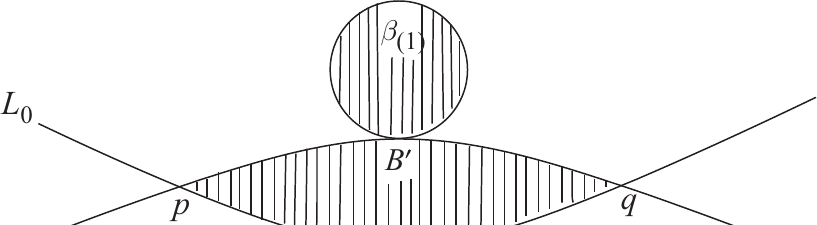
\includegraphics[width=.68\textwidth]{chapters/ch16-monotone-lagrangian-floer/figures/figure-16-3.png}
 \caption{余维 $1$ 的层 $\mathcal N(p,q;B';L_1,\beta_{(1)};J)$。}
 \label{fig:codimension-one-disc-bubble-stratum}
\end{figure}

\subsection{\termAnomaly{}与障碍}
\label{subsec:anomaly-and-obstruction}

现在研究\personFloer{} \termPreBoundaryMap{} $\partial$ 的边界性质。为此，需要分析虚维数为
$1$ 的模空间 $\mathcal M(p,q;B)$，并对每个这样的 $B$ 描述紧化模空间
$\overline{\mathcal M}(p,q;B)$ 中“余维 $1$”的奇异层。

考虑\personFloer{}流线模空间 $\widetilde{\mathcal M}(p,q;B';J)$ 及评价映射
\[
 \begin{aligned}
 \operatorname{ev}^{L_0}:\widetilde{\mathcal M}(p,q;B';J)&\to L_0,
 &(u,\tau)&\mapsto u(\tau,0),\\
 \operatorname{ev}^{L_1}:\widetilde{\mathcal M}(p,q;B';J)&\to L_1,
 &(u,\tau)&\mapsto u(\tau,1).
 \end{aligned}
\]
再考虑 $\mathcal M_1(L_0;\beta_{(0)};J_0)$、
$\mathcal M_1(L_1;\beta_{(1)};J_1)$ 及评价映射
\[
 \operatorname{ev}_0:\mathcal M_1(L_0;\beta_{(0)};J_0)\to L_0,
 \qquad
 \operatorname{ev}_1:\mathcal M_1(L_1;\beta_{(1)};J_1)\to L_1.
\]
下列集合描述 $\overline{\mathcal M}(p,q;B;J)$ 的余维 $1$ 层。

\begin{definition}
\label{def:disc-bubble-boundary-strata}
设 $p,q\in L_0\cap L_1$、$B'\in\pi_2(p,q)$，并且
$\beta_{(0)}\in G(L_0;\omega)$、$\beta_{(1)}\in G(L_1;\omega)$。对
$i=0,1$，令
\[
 \mathring{\mathcal N}(p,q;B':L_0,\beta_{(0)};J)
 =\widetilde{\mathcal M}(p,q;B';J)_{\operatorname{ev}^{L_0}}
 \!\times_{\operatorname{ev}_0}\mathcal M_1(L_0;\beta_{(0)};J_0)/\mathbb R,
\]
\[
 \mathring{\mathcal N}(p,q;B':L_1,\beta_{(1)};J)
 =\widetilde{\mathcal M}(p,q;B';J)_{\operatorname{ev}^{L_1}}
 \!\times_{\operatorname{ev}_1}\mathcal M_1(L_1;\beta_{(1)};J_1)/\mathbb R.
\]
见图\ref{fig:codimension-one-disc-bubble-stratum}。定义模空间
$\mathcal N(p,q;B':L_1,\beta_{(1)};J)$ 为
$\mathring{\mathcal N}(p,q;B':L_1,\beta_{(1)})$ 在
$\overline{\mathcal M}(p,q;B;J)$ 中的闭包，其中 $B=B'\#\beta_{(1)}$。
$\mathcal N(p,q;B':L_0,\beta_{(0)};J)$ 的定义类似，故略去。
\end{definition}

再定义
\begin{equation}
 \mathcal N([\ell_p,w],[\ell_q,w']:L_1;J)
 :=\bigcup_{\substack{(B',\beta_{(1)});\\
 [\ell_p,w]\#(B'\#\beta_{(1)})=[\ell_q,w']}}
 \mathcal N(p,q;B':L_1,\beta_{(1)};J),
\label{eq:total-disc-bubble-stratum}
\end{equation}
并类似定义 $\mathcal N([\ell_p,w],[\ell_q,w']:L_0;J)$。

我们希望说，当 $B=B'\#\beta_{(i)}$ 时，
$\mathcal N(p,q,B':L_i,\beta_{(i)};J)$ 在 $\mathcal M(p,q;B;J)$ 中具有“余维
$1$”。对一般拉格朗日对子 $(L_0,L_1)$，即便通有地选择 $J=\{J_t\}$，这句话也没有
意义。不过，若 $(L_0,L_1)$ 单调（更一般地，若它们半正且
$\mu_L(\beta_{(i)})\neq0$），则对通有选择的 $J$，情况确实如此。

\begin{theorem}
\label{thm:boundary-of-index-two-floer-moduli}
设 $L_0,L_1$ 单调，$J_0,J_1\in\mathcal J_\omega^0(L_0,L_1)$，并且
$J\in\mathfrak j^{\mathrm{reg}}_{(L_0,L_1)}(J_0,J_1)$ 如上。设
$p,q\in L_0\cap L_1$、$B\in\pi_2(p,q)$ 满足
\begin{equation}
 \mu(p,q;B)=2.
\label{eq:index-two-class}
\end{equation}
则：
\begin{enumerate}[label=(\arabic*)]
\item $\mathcal N(p,q;B':L_i,\beta_{(i)};J)$ 或者为空，或者是如下类型的紧零维
流形：
\[
 p=q,\qquad B'=0,\qquad\mu(\beta_{(i)})=2,
\]
它由位形 $u\#w$ 组成，其中 $u\equiv p$，而 $w$ 是经过 $p$ 的
$J_i$-全纯圆盘；
\item $\mathcal M(p,q;B;J)$ 是光滑一维流形，其边界是下列并：
\begin{equation}
\begin{aligned}
&\bigcup_{\substack{r\in L_0\cap L_1;\\B_1\#B_2=B}}
 \mathcal M(p,r;B_1;J)\#\mathcal M(r,q;B_2;J)\\
&\quad\cup
 \bigcup_{\substack{(B',\beta_{(1)});\\
 [\ell_p,w]\#(B'\#\beta_{(0)})=[\ell_q,w']}}
 \mathcal N(p,q;B':L_0,\beta_{(0)};J)\\
&\quad\cup
 \bigcup_{\substack{(B',\beta_{(1)});\\
 [\ell_p,w]\#(B'\#\beta_{(1)})=[\ell_q,w']}}
 \mathcal N(p,q;B:L_1,\beta_{(1)};J),
\end{aligned}
\label{eq:index-two-moduli-boundary}
\end{equation}
其中 $\mu(p,r;B_1)=\mu(r,q;B_2)=1$，且
$\mu(\beta_{(i)})=2$（$i=0,1$）。
\footnote{译者注：原书式 (16.4.6) 的第二个并（$L_0$ 项）仍以
$(B',\beta_{(1)})$ 为求并指标，而第三个并的被并对象写作
$\mathcal N(p,q;B:L_1,\beta_{(1)};J)$，不是与条件相应的 $B'$。译文逐项照录。}
\end{enumerate}
\end{theorem}

\begin{proof}
结论仍由基于模空间及评价映射横截性的维数计算得到。

先证 (1)。只考虑 $i=1$；$i=0$ 相同。依定义，
$\mathcal N(p,q;B':L_1,\beta_{(1)};J)$ 是纤维积
\[
 \frac{\widetilde{\mathcal M}(p,q;B';J)_{\operatorname{ev}^{L_1}}
 \times_{\operatorname{ev}_1}\mathcal M_1(L_1;\beta_{(1)};J_1)}{\mathbb R}
 =\frac{(\operatorname{ev}^{L_1}\times\operatorname{ev}_1)^{-1}(\Delta)}
 {\mathbb R},
\]
其中 $\Delta\subset L_1\times L_1$ 是对角线。回忆
\[
 \operatorname{vir.dim}\mathcal M_{(0;0,1)}(p,q;B')=\mu(p,q;B')-1,
\]
\[
 \operatorname{vir.dim}\mathcal M_1(L_1,J_1;\beta_{(1)})
 =n+\mu(\beta_{(1)})-2,
\]
且
\[
 \mu(p,q;B)=\mu(p,q;B')+\mu(\beta_{(1)}).
\]
由 $\mu(B)=2$，
\[
 \mu(p,q;B')=2-\mu(\beta_{(1)}),
\]
而 $\widetilde{\mathcal M}(p,q;B';J)$ 的横截性给出
$\mu(p,q;B')\geq0$。

若 $\Sigma_{L_1}\geq3$，这立即导致矛盾，故
$\mathcal N(p,q;B':L_1,\beta_{(1)})=\varnothing$。$i=0$ 亦同。因此，若
$\Sigma_{L_i}\geq3$，则 $\mathcal M(p,q;B;J)$ 是紧一维流形，边界只有分裂流线
类型。

现在考虑 $\Sigma_{L_1}=2$。此时可能有
$\mu(p,q;B')=0$、$\mu(\beta_{(1)})=2$。再次由
$\widetilde{\mathcal M}(p,q;B';J)$ 的横截性，这只有在
\[
 p=q,\qquad B'=0
\]
时发生。

\begin{remark}
\label{rem:constant-strip-with-disc-bubble-stable}
此时相伴映射 $u$ 是常值映射 $u\equiv p$。要强调的是，节点曲线
\[
 u\#w,\qquad [u]=0,\quad[w]=\beta_{(1)}
\]
是稳定映射。这是因为分支 $u\equiv p:\mathbb R\times[0,1]\to M$ 带有一个额外
特殊点 $z_0=(\tau_0,1)\in\mathbb R\times\{1\}$，气泡分支 $w$ 在此黏附。由于
$\mathbb R\times[0,1]\setminus\{z_0\}$ 共形同构于
$D^2\setminus\{1,-1,\sqrt{-1}\}$，常值分支 $u$ 定义稳定映射，故该位形是紧化\personFloer{}模空间 $\overline{\mathcal M}(p,q;B)$（其中
$B=B'\#\beta_{(1)}$）中容许的节点曲线。

\emph{应指出，到目前为止，上述论证没有使用圆盘模空间
$\mathcal M(L_i;\beta_{(i)})$ 的任何横截性断言，只使用了\personFloer{}流线模空间的
横截性}。
\end{remark}

由 $\Sigma_{L_1}=2$，$\mathcal M(L_1;\beta_{(1)};J_1)$ 的每个元素必\termSomewhereInjective{}。事实上，若
$v\in\mathcal M(L_1;\beta_{(1)};J_1)$ 不\termSomewhereInjective{}，则
[KOh00]、[Laz00] 中伪全纯圆盘的像结构定理蕴含存在
$v_i$（$i=1,\ldots,a$，$a\geq2$），使
$\sum_{i=1}^a[v_i]=[v]$，且 $\mathcal M(L_1;[v_i];J_1)$ 非空。这不可能，因为
$\mu_{L_1}(v_i)>0$。故对
$J_1\in\mathcal J_{L_1}(L_0\cap L_1)$，
$\mathcal M_1(L_1;\beta_{(1)};J_1)$ 光滑且维数为 $n-1$。

回忆，对通有选择的 $J$，评价映射
\[
 \operatorname{ev}^{L_1}\times\operatorname{ev}_1:
 \widetilde{\mathcal M}([\ell_p,w],[\ell_q,w''])
 \times\mathcal M_1(L_1;\beta_{(1)};J_1)/\mathbb R
 \longrightarrow L_1\times L_1
\]
在每个对子 $(u,w)$ 处都横截于对角线
$\Delta\subset L_1\times L_1$，其中 $w$ 是\termSomewhereInjective{}的
$J_1$-全纯映射。于是，由第 15.5 节的粘合定理，模空间
$\mathcal M(p,q;B;J)$ 成为紧光滑一维流形，其边界由
\eqref{eq:index-two-moduli-boundary} 给出。
\end{proof}

由配边论证，定理\ref{thm:boundary-of-index-two-floer-moduli} 蕴含恒等式
\begin{equation}
\begin{aligned}
0={}&\bigl\langle(\partial\circ\partial)([\ell_p,w]),[\ell_q,w']\bigr\rangle
 +\#\mathcal N([\ell_p,w],[\ell_q,w']:L_0)\\
&+\#\mathcal N([\ell_p,w],[\ell_q,w']:L_1),
\end{aligned}
\label{eq:boundary-square-with-anomaly-strata}
\end{equation}
其中
$\langle(\partial\circ\partial)([\ell_p,w]),[\ell_q,w']\rangle$ 表示
$(\partial\circ\partial)([\ell_p,w])$ 中 $[\ell_q,w']$ 的系数，而 $\#$ 是带符号的
阶数。

下面推导\eqref{eq:boundary-square-with-anomaly-strata} 的后果。分成两种情形：
\begin{enumerate}[label=(\arabic*)]
\item $L_0,L_1$ 都有 $\Sigma_{L_i}>2$；
\item $L_0,L_1$ 中有一个或两个的\termMinimalMaslovNumber{}为 $2$。
\end{enumerate}

先考虑 (1)。若 $\beta_{(i)}\in\pi_2(M;L_i)$ 满足 $\mu(\beta_{(i)})>2$，则当
$\mu([\ell_q,w'])-\mu([\ell_p,w])=2$ 时，对通有选择的 $\{J_t\}_t$，有
$\mathcal N([\ell_p,w],[\ell_q,w']:L_i)=\varnothing$。据此，
\eqref{eq:boundary-square-with-anomaly-strata} 中来自 $\mathcal N$ 的贡献由维数计算变为
零，从而证明如下定理。

\begin{theorem}
\label{thm:minimal-maslov-at-least-three-floer-homology}
设 $L_0,L_1$ 是单调拉格朗日子流形，且对 $i=0,1$ 有 $\Sigma_{L_i}\geq3$。
则\personFloer{} \termPreBoundaryMap{}
\[
 \partial:CF_R^*(L_1,L_0;\ell_0)\longrightarrow CF_R^{*+1}(L_1,L_0;\ell_0)
\]
是边界映射，即满足 $\partial\circ\partial=0$。特别地，可以定义\personFloer{}同调
\[
 HF(L_1,L_0;\ell_0)=\ker\partial/\operatorname{Im}\partial.
\]
这里，当 $L_0,L_1$ 相对 spin 时取底系数环 $R=\mathbb Z$，一般取
$R=\mathbb Z_2$。
\end{theorem}

现在研究情形 (2)，即 $L_1$ 或 $L_0$ 的\termMinimalMaslovNumber{}为 $2$。再次由
维数计算，$\partial\circ\partial$ 的矩阵元为
\[
\begin{aligned}
 \bigl\langle(\partial\circ\partial)([\ell_p,w]),[\ell_q,w']\bigr\rangle
 ={}&-\#\mathcal N([\ell_p,w],[\ell_q,w']:L_0)\\
 &-\#\mathcal N([\ell_p,w],[\ell_q,w']:L_1).
\end{aligned}
\]
回忆，只有当
\[
 p=q,\qquad B'=0,\qquad
 \mu(\beta_{(0)})=2=\mu(\beta_{(1)}),
\]
且相伴圆盘分支位形经过 $p$ 时，对子 $(B',\beta_{(0)})$ 或
$(B',\beta_{(1)})$ 才对右端的和有非平凡贡献。

\begin{lemma}
\label{lem:disc-bubble-stratum-count}
设 $i=0,1$，$[\ell_p,w]$ 如上。则
\begin{equation}
 \#\mathcal N([\ell_p,w],[\ell_p,w']:L_i)=\Phi(L_i;\{\mathrm{pt}\}).
\label{eq:disc-bubble-count-one-point-invariant}
\end{equation}
特别地，它不依赖于 $p\in L_0\cap L_1$，而依赖于 $L_i$（$i=0,1$）。此外，若
$[q,w']=[p,w]\#B$，且当 $B=B'\#\beta_{(i)}$ 时
$\#\mathcal N(p,q;B':L_i,\beta_{(i)};J)\neq0$，则
\begin{equation}
 \omega(w')-\omega(w)=\omega(\beta_{(i)}).
\label{eq:disc-bubble-area-difference}
\end{equation}
\end{lemma}

\begin{proof}
回忆\eqref{eq:total-disc-bubble-stratum} 中
$\mathcal N([\ell_p,w],[\ell_p,w']:L_i)$ 的定义。依定义，
\[
 \mathcal N(p,q;B':L_i,\beta_{(i)};J)
 =\mathcal M_{(0;1;0)}(p,p;0;J)_{\operatorname{ev}}
 \times_{\operatorname{ev}}\mathcal M_1(L_i;\beta_{(i)};J_i)/\mathbb R.
\]
$\mathcal M_{(0;1;0)}(p,p;0;J)$ 中每个元素的映射分支均为常值，所以
\[
 \mathcal M_{(0;1;0)}(p,p;0;J)/\mathbb R
 \cong\{p\}\times
 \{(\tau,1)\in\mathbb R\times[0,1]\mid\tau\in\mathbb R\}/\mathbb R
 \cong\mathcal M_{0;(0,3)},
\]
其中 $\mathcal M_{0;(0,3)}$ 是边界上带三个标记点的亏格零\personDeligne{}--\personMumford{}模空间，因而只有一个点。而且 $\mathbb R$ 在因子
$\mathcal M_1(L_i;\beta_{(i)};J_i)$ 上作用平凡，故
\[
 \widetilde{\mathcal M}(p,p;0;J)_{\operatorname{ev}}
 \times_{\operatorname{ev}}\overline{\mathcal M}_1(L_i;\beta_{(i)};J_i)/\mathbb R
 \cong\{p\}\times_{\operatorname{ev}_\beta}
 \mathcal M_1(L_i;\beta_{(i)};J_i).
\]
但由 $\Phi(L_i;\{\mathrm{pt}\})$ 的定义，
\[
 \Phi(L_i;\{p\})
 =\sum_{\beta_{(i)}\in\pi_2(L_i)}
 \#\bigl(\mathcal M_1(L_i;\beta_{(i)};J_i)_{\operatorname{ev}_\beta}
 \times\{p\}\bigr).
\]
结合引理\ref{lem:one-point-count-invariance}，即得
\eqref{eq:disc-bubble-count-one-point-invariant}。

为证明\eqref{eq:disc-bubble-area-difference}，对任意
$u\in\mathcal M([\ell_p,w],[\ell_p,w'];J)$，同伦条件 $w\#u\simeq w'$ 先给出
\[
 \omega(B)=\omega(w')-\omega(w).
\]
辛面积在\personGromov{}--\personFloer{}极限下保持，故
\eqref{eq:disc-bubble-area-difference} 成立。
\end{proof}

该引理给出，对所有 $p\in L_0\cap L_1$，
\[
 \sum_{[w']\in\pi_2(p;\ell_0)}
 \bigl\langle(\partial\circ\partial)([\ell_p,w]),[\ell_p,w']\bigr\rangle
 =\pm\bigl(\Phi(L_1;\{\mathrm{pt}\})-\Phi(L_0;\{\mathrm{pt}\})\bigr).
\]
（符号可以唯一确定，证明留给有兴趣的读者。）进一步，若对 $i=0$ 或 $1$，
$B=B'\#\beta_{(i)}$ 且
$\mathcal N(p,p,B':L_i,\beta_{(i)})\neq\varnothing$，则有
$[\ell_p,w']=g_i\cdot[\ell_p,w]$，其中
$g_i\in G(L_i;\omega)$ 依赖于是哪一个 $i$。因此
\[
 \partial\circ\partial([\ell_p,w])
 =\pm\bigl(\Phi(L_1;\{\mathrm{pt}\})g_1\cdot[\ell_p,w]
 -\Phi(L_0;\{\mathrm{pt}\})g_0\cdot[\ell_p,w]\bigr).
\]

由命题\ref{prop:monotone-lagrangian-group-rank-one}，对任意单调 $L$，
$G(L;\omega)$ 是秩为 $1$ 的自由\personAbel{}群。把 $G(L;\omega)$ 写成乘法群，相伴\personNovikov{}环可写成\personLaurent{}多项式环
\[
 \Lambda(L;\ell_0)\cong R[T^a],
\]
\footnote{译者注：原书称其为\personLaurent{}多项式环，却只写 $R[T^a]$，没有显示
$T^{-a}$；译文照录。}
其中 $T$ 是形式参数，$a>0$ 是周期群
$\Gamma(L;\omega)=I_\omega(G(L;\omega))$ 的正生成元。此外，每个满足
$\mu(\beta)=2$ 的 $\beta\in\pi_2(M,L)$ 都投影到
$G(L;\omega)$ 中的同一个元素 $T^a$。

用此记号，若对 $i=0$ 或 $1$，$B=B'\#\beta_{(i)}$ 且
$\mathcal N(p,p,B':L_i,\beta_{(i)})\neq\varnothing$，则
\[
 [\ell_p,w']=T^{\omega(g_i)}[\ell_p,w].
\]
由于 $\mu(\beta_{(i)})=2$，每个这样的 $g_i$ 都必为群 $G(L_i;\omega)$ 的生成元。
概括上述讨论，得到下列定理。

\begin{theorem}
\label{thm:boundary-square-monotone-maslov-two}
设 $L_i$ 单调且 $\Sigma_{L_i}=2$。以
$a_i=\omega(\beta_{(i)})$（$i=0,1$）表示上述群
$\{\omega(\beta)\mid\beta\in\pi(M,L_i)\}$ 的生成元。则
\begin{equation}
 \partial\circ\partial[p,w]
 =\pm\bigl(\Phi(L_0;\{\mathrm{pt}\})T^{a_0}
 -\Phi(L_1;\{\mathrm{pt}\})T^{a_1}\bigr)[p,w],
\label{eq:boundary-square-scalar}
\end{equation}
其中对 $G(L_i;\omega)$ 的生成元 $g_i$ 有 $a_i=\omega(g_i)$。特别地，
$\partial\circ\partial$ 是由 $\Lambda_{\mathrm{Nov}}$ 中标量元素给出的乘法算子。
\footnote{译者注：原书定理中把相对同伦群印作 $\pi(M,L_i)$，没有下标 $2$；译文
照录。}
\end{theorem}

\begin{proof}
只需证明最后一句。这立即来自如下事实：
\[
 \Phi(L_0;\{\mathrm{pt}\})T^{a_0}
 -\Phi(L_1;\{\mathrm{pt}\})T^{a_1}
\]
不依赖于生成元 $[p,w]$，只依赖于对子 $(L_0,L_1)$ 的几何。
\end{proof}

由此可见，除非
\[
 \Phi(L_0;\{\mathrm{pt}\})T^{a_0}
 =\Phi(L_1;\{\mathrm{pt}\})T^{a_1},
\]
否则 $\partial\circ\partial\neq0$。

\begin{corollary}
\label{cor:criterion-boundary-square-zero}
设 $(L_0,L_1)$ 是 $(M,\omega)$ 上的单调拉格朗日子流形对，$a_i$ 如上。则
$\partial\circ\partial=0$ 当且仅当
\[
 \Phi(L_0;\{\mathrm{pt}\})=\Phi(L_1;\{\mathrm{pt}\}),
 \qquad a_0=a_1.
\]
\footnote{译者注：按紧邻的标量等式，若两个单点不变量同时为零，则无需
$a_0=a_1$ 也有 $\partial^2=0$；原书此处的“当且仅当”似乎缺少非零性条件。译文
照录结论。}
\end{corollary}

该结果是 (Oh95a) 的一个轻微加强，也是 (FOOO09) 命题 3.7.17 的特例；后者在形变\personFloer{}（上）同调的更一般背景中以势函数 $\mathfrak{PO}$ 陈述了类似判据。当前情形
对应未形变单调情形，即 (FOOO09) 命题 3.7.17 中形变参数 $b_0=0=b_1$ 的情形。

上述推论结合单点 GW 不变量的辛不变性，蕴含作者在 (Oh93a) 中得到的下列结果。

\begin{theorem}
\label{thm:hamiltonian-image-monotone-floer-invariance}
设 $L$ 是紧单调拉格朗日子流形，$\Sigma_L\geq2$。令 $L_0=L$、
$L_1=\phi(L)$，其中 $\phi$ 是使 $\phi(L)$ 与 $L$ 横截相交的哈密顿微分同胚。则\personFloer{}同调 $HF(L,\phi(L))$ 有良定义，并在改变 $\phi$ 时保持不变。
\end{theorem}

后一不变性可通过非自治\personCauchy{}--\personRiemann{}方程 (14.4.45) 构造链映射来证明。由于该
方程不具有平移对称性，相伴模空间的自同构群平凡，所以需要考察维数为 $0,1$ 的模
空间，而非像\personFloer{}边界映射的模空间那样考察维数 $1,2$ 的模空间。

尽管如此，对边界映射模空间的类似分析也适用于链映射模空间，并证明下列定理。

\begin{theorem}
\label{thm:monotone-continuation-chain-isomorphism}
设 $(L_0,L_1)$ 是单调对。则 (14.4.44) 的模空间在维数为 $0$ 或 $1$ 时紧。特别地，
若对子 $(L_0,L_1)$ 的\personFloer{} \termPreBoundaryMap{}是边界，即满足 $\partial^2=0$，
则存在链同构
\[
 h_{\phi_{(0)}\phi_{(1)}}:CF_*(L_0,L_1)
 \longrightarrow CF_*(\phi_{(0)}^1(L_0),\phi_{(1)}^1(L_1)).
\]
特别地，
\[
 HF_*(L_0,L_1)
 \cong HF_*(\phi_{(0)}^1(L_0),\phi_{(1)}^1(L_1)).
\]
\end{theorem}

\begin{exercise}
\label{ex:prove-monotone-chain-isomorphism}
证明该定理。（证明见 (Oh93a, Oh96c)。）
\end{exercise}
